%%%%%%%% ICML 2018 EXAMPLE LATEX SUBMISSION FILE %%%%%%%%%%%%%%%%%

\documentclass{article}

% Recommended, but optional, packages for figures and better typesetting:
\usepackage{microtype}
\usepackage{graphicx}
\usepackage{subfigure}
\usepackage{booktabs} % for professional tables

% hyperref makes hyperlinks in the resulting PDF.
% If your build breaks (sometimes temporarily if a hyperlink spans a page)
% please comment out the following usepackage line and replace
% \usepackage{icml2018} with \usepackage[nohyperref]{icml2018} above.
\usepackage{hyperref}

% Attempt to make hyperref and algorithmic work together better:
\newcommand{\theHalgorithm}{\arabic{algorithm}}

% Use the following line for the initial blind version submitted for review:
%\usepackage{icml2018_ift6269}

% If accepted, instead use the following line for the camera-ready submission:
\usepackage[accepted]{icml2018_ift6269}
% SLJ: -> use this for your IFT 6269 project report!

% The \icmltitle you define below is probably too long as a header.
% Therefore, a short form for the running title is supplied here:
\icmltitlerunning{IFT6759 - Advanced ML Projects - Final Report}

\begin{document}

\twocolumn[
\icmltitle{Multimodal Emotion Prediction in Group Conversation}

% It is OKAY to include author information, even for blind
% submissions: the style file will automatically remove it for you
% unless you've provided the [accepted] option to the icml2018
% package.

% List of affiliations: The first argument should be a (short)
% identifier you will use later to specify author affiliations
% Academic affiliations should list Department, University, City, Region, Country
% Industry affiliations should list Company, City, Region, Country

% You can specify symbols, otherwise they are numbered in order.
% Ideally, you should not use this facility. Affiliations will be numbered
% in order of appearance and this is the preferred way.
\icmlsetsymbol{equal}{*}

\begin{icmlauthorlist}
\icmlauthor{TOMA ALLARY,}{}
\icmlauthor{THIERRY BÉDARD-CORTEY,}{}
\icmlauthor{PHILIPPE BERGERON,}{}
\icmlauthor{YUAN LI}{}
\end{icmlauthorlist}

% You may provide any keywords that you
% find helpful for describing your paper; these are used to populate
% the "keywords" metadata in the PDF but will not be shown in the document
\icmlkeywords{Machine Learning, ICML}

\vskip 0.3in
]

% this must go after the closing bracket ] following \twocolumn[ ...

% This command actually creates the footnote in the first column
% listing the affiliations and the copyright notice.
% The command takes one argument, which is text to display at the start of the footnote.
% The \icmlEqualContribution command is standard text for equal contribution.
% Remove it (just {}) if you do not need this facility.

%\printAffiliationsAndNotice{}  % leave blank if no need to mention equal contribution
% \printAffiliationsAndNotice{\icmlEqualContribution} % otherwise use the standard text.

\begin{abstract}
Emotion prediction in group conversations is a challenging task due to the complexity of human interactions and the multimodal nature of emotional expressions.This project aims to develop a multimodal model that integrates textual and audio features for emotion prediction in group conversations. It combines RoBERTa for text embeddings, WavLM for audio embeddings, and a transformer-based fusion layer to enhance emotion recognition. The project is based on the study "Emotional Cues Extraction and Fusion for Multi-modal Emotion Prediction and Recognition in Conversation"[1].
\end{abstract}

\section{Introduction}
Human emotions are important for the  communication. In recent years, deep learning has been achieving tremendous success on numerous machine learning
applications. In natural language and speech processing areas, conversational AI had a huge growth in recent years — from virtual assistants to customer support chatbots. But there’s still a big gap: most systems don’t understand how we feel.
That’s why emotion-aware systems are so valuable — they enable more natural, empathetic, and human-like interactions. In this project, Our goal is to  build a multimodal machine learning model that could predict the next emotion in a group conversation using traces of previous audio and text. More specifically, we explore simplified architectures to improve on current existing models that are complex and heavy to train and implement. Light and re-usable architecture are generally more suited for real-life tasks where cost and time are important. This work could serve as the basis for applications such as social robots, therapeutic robots and intelligent tutoring systems. 

\colorbox{yellow}{TODO: add contribution}\\

\section{Relate Work}
There are three major approaches commonly used in emotion detection models.
First is RNN-based models, which are good for temporal sequences but suffer with long-term dependencies and slow processing. 
The second is Transformer-based models, which excel at capturing long-range dependencies and can process data in parallel — though they are resource-intensive.
The third is Graph-based models, which represent conversations as interactions between speakers, allowing them to infer emotions based on relationships. These models are powerful but often complex to implement.
Our project mainly leveraged transformer-based models for their strong performance on language and speech tasks.

 This study \cite{ERCFusionModel} explores the extraction and fusion of emotional cues from multiple modalities, including text and audio, to enhance emotion prediction in conversations. The authors propose a transformer-based fusion layer to combine embeddings from different modalities, achieving state-of-the-art results in emotion recognition tasks.
 
\subsection{RoBERTa}
RoBERTa (Robustly Optimized BERT Pretraining Approach)  \cite{liu2019roberta}is a transformer-based language model developed by Facebook AI. This model significantly enhances the original BERT architecture through several key modifications in its pre-training methodology. Unlike BERT, RoBERTa was trained on a substantially larger dataset, totaling 160 GB of diverse text and code. This extensive training corpus allowed the model to develop a more robust and generalized understanding of language. One of the critical improvements in RoBERTa is the removal of the Next Sentence Prediction (NSP) objective used in BERT, which was found to not consistently improve downstream task performance. Additionally, RoBERTa employs dynamic masking during pre-training, where the masked tokens change in each epoch, forcing the model to learn more effectively from different parts of the input. The model also benefits from being trained with much larger batch sizes, contributing to more stable and efficient learning. RoBERTa's architecture, being based on the transformer, inherently excels at capturing long-range dependencies within text, making it particularly adept at understanding context. In dialogue, emotions are often conveyed subtly and are deeply intertwined with the surrounding linguistic context. RoBERTa's enhanced semantic capabilities, stemming from its extensive training and architectural refinements, enable it to discern these intricate relationships and make more accurate emotion predictions by considering the nuances of the conversational flow and the interplay of words.

\subsection{WavLM}
WavLM \cite{chen2021wavlm}, short for Waveform Language Model, represents a significant advancement in self-supervised learning for comprehensive speech processing, developed by Microsoft. This large-scale model is meticulously engineered to learn rich, universal representations directly from raw audio waveforms, eliminating the need for extensive manual feature engineering. Building upon the success of the wav2vec 2.0 framework, WavLM introduces innovative techniques to further enhance the quality of learned representations. A key contribution of WavLM is its emphasis on capturing prosodic features like tone, rhythm, and pitch – elements that carry crucial information about a speaker's emotional state. By explicitly modeling these acoustic characteristics, WavLM gains a distinct advantage in tasks such as emotion analysis, where these subtle vocal cues are paramount. Beyond emotional understanding, WavLM demonstrates its versatility by supporting a wide array of speech-related tasks, including speaker identification, automatic speech recognition, and emotion recognition. This broad applicability makes WavLM an exceptionally valuable component for multimodal fusion approaches, where information from different modalities, such as audio and text, can be combined to achieve a more holistic and accurate understanding of communicative signals. Its ability to extract meaningful features from raw audio across various tasks underscores its potential to significantly improve the performance of speech-centric artificial intelligence systems.


\section{ Task Definition}
Emotion Prediction in Conversation (\textbf{EPC}) In a multi-modal
multi-party (or dyadic) dialogue containing text and audio
$\mathrm{D} = {(u_1, s_1), (u_2, s_2), ..., (u_N, s_N)}$, where $(u_i, s_i)$ represents
the ith utterance-speaker pair in the conversation, N is
the number of utterances in the dialogue. EPC aims to predict
the emotion category label $emotion_{n+1}$ of the future utterance
speaker pair ($u_{n+1}, s_{n+1}$) by given the historical dialogues
${(u_1, s_1), (u_2, s_2), ..., (u_n, s_n)}$.

\subsection{Dataset}
MELD is a popular dataset for
tasks involving the analysis of emotions expressed by multiple
speakers. It encompasses a collection of over 1400 dialogues
and 13,000 speech instances extracted from the television show
Friends. Emotion annotation in the dataset includes: neutral,
happiness, surprise, sadness, anger, disgust, and fear.

\section{Method}
\subsection{Data Preprocess and Feature Extraction}

In this project, we used a multimodal feature extraction method that combines both audio and text information to better predict emotions.

For audio features, we used a pre-trained model called WavLM (wavlm-base-plus) from Hugging Face. First, the audio files (in .mp4 format) were loaded and converted into raw waveforms. These waveforms were then passed into WavLM to generate hidden representations. The output from WavLM captures important speech characteristics like tone, pitch, speaking style, and voice quality, all of which are helpful for recognizing emotions.

For text features, we used the RoBERTa-base model. We read the utterances from a CSV file, then used the RoBERTa tokenizer to split each sentence into tokens that the model can understand. After tokenization, the tokens were passed into the RoBERTa model to get sentence embeddings. These embeddings represent the meaning, sentiment, and emotional hints inside the text.

After extracting features from both audio and text separately, we combined (concatenated) them together into a single feature vector for each sample. This combined feature includes both what was said (text) and how it was said (audio), giving the model a more complete view of the emotional content.

This method allows us to use both modalities at the same time, which improves the model's ability to detect complex emotions that may not be clear from just the audio or just the text alone.

In addition, before extracting features, we combined the audio clips and merged the text utterances for each conversation. Instead of treating each utterance separately, we processed the whole conversation as a single input. For audio, we concatenated the waveform files belonging to the same dialogue into one long audio sequence. For text, we joined the utterances from the same conversation into one long text string. This way, the models could capture the full context of the conversation — including how emotions develop over time — rather than just focusing on isolated sentences. After combining, we extracted features from the full conversation-level audio and text, and then fused them together for downstream emotion prediction.

\colorbox{yellow}{TODO: add image}\\

\subsection{Reference baseline method}

Our baseline architecture is from study \cite{ERCFusionModel}.
As seen in Figure \ref{fig:BaselineArchitecture}, they propose an architecture using both text and audio modalities. They also extract a mel-spectrogram as a third modality from the audio. Their first steps are to extract features from modalities using pre-trained models (i.e. RoBERTa, WaveLM and a Spectrum Extraction Tool)

\begin{figure}[htbp]
  \centering
  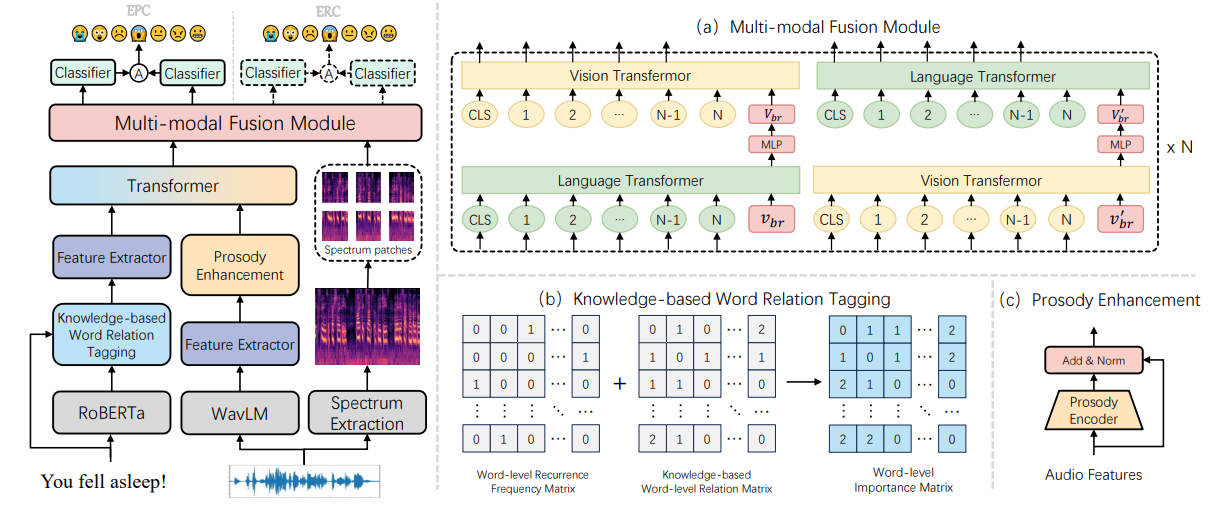
\includegraphics[width=0.5\textwidth]{Images/EPCFusion_BaselineArchitecture.png}
  \caption{\textit{Schema of the baseline architecture. The left side is the main framework of the model. (a) multi-modal fusion module, the green part represents the pre-trained
language transformer layer, the yellow part represents the pre-trained vision transformer layer, the pink part is trainable, and other
parts are frozen.}}
  \label{fig:BaselineArchitecture}
\end{figure}

\subsubsection{KWRT}
On textual side, they add a bloc of Knowledge-Based Word Relation Tagging (KWRT) before extracting their features. This block aims to give more word relation cues that context alone could not provide. This technique leverage external resources to identifies relationship between two words. Usually this is done through some human involvement in the labelling or learning process. In their specific use-case, their architecture use ConceptNet \cite{speer2018conceptnet}, a knowledge graph that connects words and phrases of natural language with labeled edges.

\subsubsection{Prosody Enhancement}
As for the waveform, the second modality, they use what they call a "Prosody Enhancement". Prosody is the study of intonation, stress and rhythm of spoken audio. They enhance the emotional cues given by the audio through a fine-tuned encoder \cite{yang2022speech}. Their claim is that this module extract and amplify emotional cues.

\subsubsection{Transformer module}
\colorbox{yellow}{TODO: explain Transformer module}\\

\subsubsection{Fusion module}
\colorbox{yellow}{TODO: explain fusion module}\\



\subsection{First architecture draft}
Even though the baseline model yield respectable results, having such complexity and that many components can be complex to implement, train and deploy. Hence, our main idea is to build a simpler architecture that result in similar performance with fewer parameters and less complexity.

\begin{figure}[htbp]
  \centering
  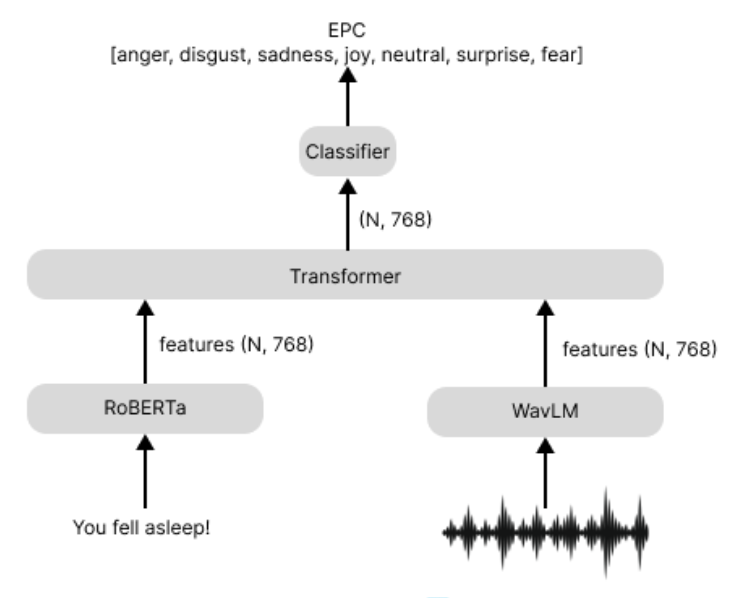
\includegraphics[width=0.5\textwidth]{Images/architecture_draft.png}
  \caption{\textit{First draft of our proposed simplified architecture illustrating the core modules used where $N$ is the length of extracted features sequence.}}
  \label{fig:DraftArchitecture}
\end{figure}

We decided to remove some of the proposed modules to keep only the core modules that can grasp the context of a conversation. Intuitively, we pruned the spectrogram extraction, the third modality, as WaveLM already has a significant capacity to treat the audio cues.
Also, KWRT and Prosody Enhancement modules are not in our proposal, see Figure \ref{fig:DraftArchitecture}. This first draft is however not really detailed and require specific solution to fuse both modalities without losing each extracted features. In Figure \ref{fig:DraftArchitecture}, we supposed $N$ is fixed, but in reality, $N$ differ for each conversation and even between both modalities. The next sections cover three different approaches we developed in parallel to tackle these issues and compare the results.


\subsection{Convolution Neural Network}
Our first approach
\colorbox{yellow}{TODO}\\

\subsection{Decoder Transformer \& MLP}
\colorbox{yellow}{TODO}\\

\subsection{Encoder Transformer \& MLP}
\colorbox{yellow}{TODO}\\


\section{Experiments}
For our experiments, we utilize pre-trained wavLM and RoBERTa
models to extract 768-dimensional features, then use serval different architectures to predict next emotion.
architecture 1
architecture 2
architecture 3
\\ \colorbox{yellow}{TODO:}\\
\textit{Experiments: Comparisons to baselines using metrics (explain what the metrics are), with visualizations in terms of graphs, tables etc. (if you can show more, e.g., qualitative results with images - the better).}\\


\section{Optional sections if needed}

\subsection{Figures}

You may want to include figures in the paper to illustrate
your approach and results. Such artwork should be centered,
legible, and separated from the text. Lines should be dark and at
least 0.5~points thick for purposes of reproduction, and text should
not appear on a gray background.

Label all distinct components of each figure. If the figure takes the
form of a graph, then give a name for each axis and include a legend
that briefly describes each curve. Do not include a title inside the
figure; instead, the caption should serve this function.

Number figures sequentially, placing the figure number and caption
\emph{after} the graphics, with at least 0.1~inches of space before
the caption and 0.1~inches after it, as in
Figure~\ref{icml-historical}. The figure caption should be set in
9~point type and centered unless it runs two or more lines, in which
case it should be flush left. You may float figures to the top or
bottom of a column, and you may set wide figures across both columns
(use the environment \texttt{figure*} in \LaTeX). Always place
two-column figures at the top or bottom of the page.

\subsection{Algorithms}

If you are using \LaTeX, please use the ``algorithm'' and ``algorithmic''
environments to format pseudocode. These require
the corresponding stylefiles, algorithm.sty and
algorithmic.sty, which are supplied with this package.
Algorithm~\ref{alg:example} shows an example.

\begin{algorithm}[tb]
   \caption{Bubble Sort}
   \label{alg:example}
\begin{algorithmic}
   \STATE {\bfseries Input:} data $x_i$, size $m$
   \REPEAT
   \STATE Initialize $noChange = true$.
   \FOR{$i=1$ {\bfseries to} $m-1$}
   \IF{$x_i > x_{i+1}$}
   \STATE Swap $x_i$ and $x_{i+1}$
   \STATE $noChange = false$
   \ENDIF
   \ENDFOR
   \UNTIL{$noChange$ is $true$}
\end{algorithmic}
\end{algorithm}

\subsection{Tables}

You may also want to include tables that summarize material. Like
figures, these should be centered, legible, and numbered consecutively.
However, place the title \emph{above} the table with at least
0.1~inches of space before the title and the same after it, as in
Table~\ref{sample-table}. The table title should be set in 9~point
type and centered unless it runs two or more lines, in which case it
should be flush left.

% Note use of \abovespace and \belowspace to get reasonable spacing
% above and below tabular lines.

\begin{table}[t]
\caption{Classification accuracies for naive Bayes and flexible
Bayes on various data sets.}
\label{sample-table}
\vskip 0.15in
\begin{center}
\begin{small}
\begin{sc}
\begin{tabular}{lcccr}
\toprule
Data set & Naive & Flexible & Better? \\
\midrule
Breast    & 95.9$\pm$ 0.2& 96.7$\pm$ 0.2& $\surd$ \\
Cleveland & 83.3$\pm$ 0.6& 80.0$\pm$ 0.6& $\times$\\
Glass2    & 61.9$\pm$ 1.4& 83.8$\pm$ 0.7& $\surd$ \\
Credit    & 74.8$\pm$ 0.5& 78.3$\pm$ 0.6&         \\
Horse     & 73.3$\pm$ 0.9& 69.7$\pm$ 1.0& $\times$\\
Meta      & 67.1$\pm$ 0.6& 76.5$\pm$ 0.5& $\surd$ \\
Pima      & 75.1$\pm$ 0.6& 73.9$\pm$ 0.5&         \\
Vehicle   & 44.9$\pm$ 0.6& 61.5$\pm$ 0.4& $\surd$ \\
\bottomrule
\end{tabular}
\end{sc}
\end{small}
\end{center}
\vskip -0.1in
\end{table}

Tables contain textual material, whereas figures contain graphical material.
Specify the contents of each row and column in the table's topmost
row. Again, you may float tables to a column's top or bottom, and set
wide tables across both columns. Place two-column tables at the
top or bottom of the page.


% In the unusual situation where you want a paper to appear in the
% references without citing it in the main text, use \nocite
\nocite{langley00}

\bibliography{example_paper}
\bibliographystyle{icml2018}



\end{document}


% This document was modified from the file originally made available by
% Pat Langley and Andrea Danyluk for ICML-2K. This version was created
% by Iain Murray in 2018. It was modified from a version from Dan Roy in
% 2017, which was based on a version from Lise Getoor and Tobias
% Scheffer, which was slightly modified from the 2010 version by
% Thorsten Joachims & Johannes Fuernkranz, slightly modified from the
% 2009 version by Kiri Wagstaff and Sam Roweis's 2008 version, which is
% slightly modified from Prasad Tadepalli's 2007 version which is a
% lightly changed version of the previous year's version by Andrew
% Moore, which was in turn edited from those of Kristian Kersting and
% Codrina Lauth. Alex Smola contributed to the algorithmic style files.
